\section{Othello}
\label{sec:othello}

Othello ist ein Brettspiel für zwei Spieler. Das schachbrettartige Spielfeld umfasst $8\times 8$ Felder. Die 64 Spielsteine sind auf der einen Seite weiß und auf der anderen Seite schwarz. Ein Spieler spielt mit der weißen Seite, der andere mit der schwarzen. Ziel ist es, am Ende des Spiels möglichst viele Steine der eigenen Farbe auf dem Spielfeld liegen zu haben.

\begin{figure}[H]
    \centering
    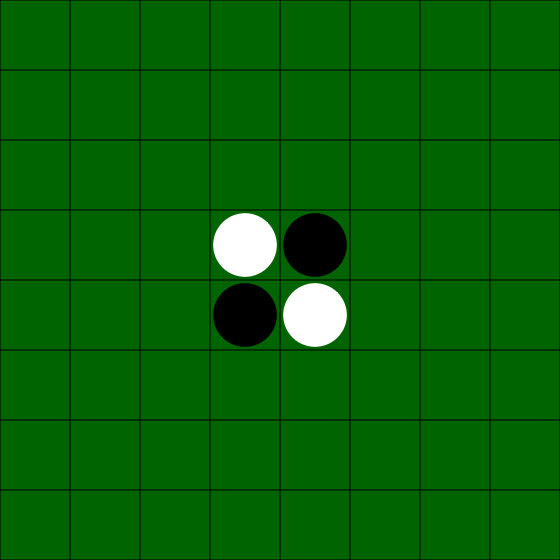
\includegraphics[width=\textwidth / 2]{board_initial}
    \caption{Initialer Spielzustand}
    \label{fig:board_initial}
\end{figure}

Zu Beginn des Spiels werden jeweils zwei Steine jedes Spielers so auf die vier mittleren Felder des Spielfelds gelegt, dass
– wie in Abbildung \ref{fig:board_initial} zu sehen – die Steine eines Spielers einander diagonal gegenüber liegen.

Die Spieler legen nun abwechselnd jeweils einen Stein ihrer eigenen Farbe auf das Spielfeld. Steine können nur auf freie
Felder gelegt werden, die in horizontale, vertikale oder diagonale Richtung an einen oder mehrere gegnerische Steine,
gefolgt von einem eigenen Stein, angrenzen. Eine beispielhafte Spielsituation, in der die möglichen Spielzüge für den
schwarzen Spieler als kleinere Kreise dargestellt werden, ist in \autoref{fig:board_possible_moves} zu sehen. 

\begin{figure}[H]
    \centering
    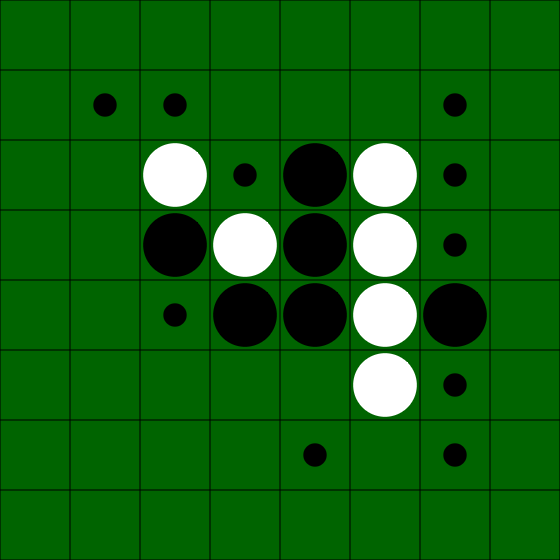
\includegraphics[width=\textwidth / 2]{board_possible_moves}
    \caption{Mögliche Züge des schwarzen Spielers}
    \label{fig:board_possible_moves}
\end{figure}

Alle gegnerischen Steine, die durch den gesetzten Stein in eine der 8 Richtungen lückenlos eingeschlossen werden, ohne dass sich freie Felder dazwischen befinden, werden umgedreht und erhalten dadurch die Farbe des Spielers, der diesen Zug ausgeführt hat.

Ist einer der Spieler zugunfähig, das heißt, er ist an der Reihe, kann jedoch keinen validen Zug spielen, so ist der
andere Spieler erneut am Zug.

Das Spiel endet, sobald beide Spieler zugunfähig sind. Der Gewinner ist dann der Spieler, der die meisten Steine seiner
Farbe auf dem Spielfeld liegen hat.
\cite{worldothellorules}
